\subsection{图表与单位}
\label{sec:figure-table}

\autoref{fig:sample} 展示了一张示例图片。

\begin{figure}[htbp]
    \centering
    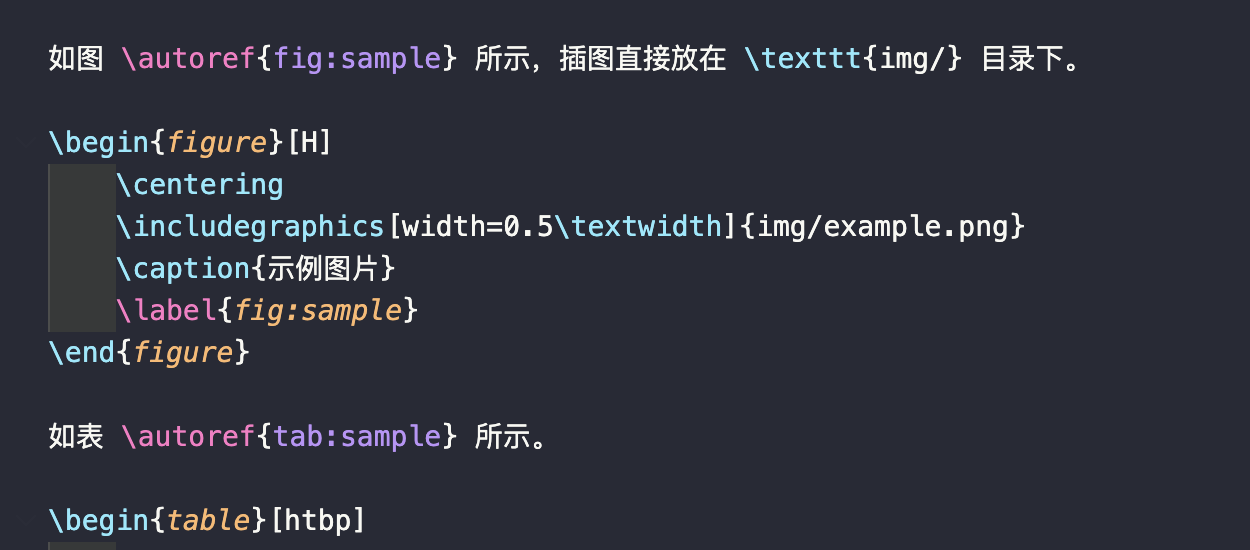
\includegraphics[width=0.5\textwidth]{img/example.png}
    \caption{示例图片}
    \label{fig:sample}
\end{figure}

\autoref{tab:params} 是一个使用 \texttt{booktabs} 的三线表。

\begin{table}[htbp]
    \centering
    \caption{系统参数}
    \begin{tabular}{ccc}
        \toprule
        参数 & 符号 & 数值 \\
        \midrule
        采样率 & $f_s$ & \SI{20}{\kilo\hertz} \\
        供电电压 & $V_{cc}$ & \SI{400}{\volt} \\
        线阻 & $R_w$ & \SI{10}{\milli\ohm} \\
        \bottomrule
    \end{tabular}
    \label{tab:params}
\end{table}

\texttt{siunitx} 提供了统一的单位排版：\SI{50}{\mega\hertz}、\SI{3.3}{\volt}、\SI{100}{\milli\ampere}。

\autoref{tab:wide} 是一个使用 \texttt{tabularx} 的宽表示例。

\newcolumntype{Y}{>{\centering\arraybackslash}X}

\begin{table}[htbp]
    \centering
    \caption{宽表参数}
    \label{tab:wide}
    \begin{tabularx}{0.85\textwidth}{YYY}
        \toprule
        参数 & 符号 & 数值 \\
        \midrule
        采样率 & $f_s$ & \SI{20}{\kilo\hertz} \\
        供电电压 & $V_{cc}$ & \SI{400}{\volt} \\
        线阻 & $R_w$ & \SI{10}{\milli\ohm} \\
        \bottomrule
    \end{tabularx}
\end{table}
